%PART_2_CHAP_1
\myChapter{M}{éthode participative}
%WAIT a Review ok
\begin{resumChap}
Pour ce premier chapitre, nous commencerons par présenter la production de ce travail de co-conception, c'est-à-dire le Kit robotique pédagogique ErgoJr.\par%
Puis, après un bref rappel sur la notion de conception centrée utilisateur, nous présenterons comment a été mis en place ce processus avec les enseignants dans les lycées, mais aussi avec d'autres partenaires, comme le rectorat ou encore au travers d'événements connexes comme des workshop ou des salons.\par%
Ensuite, nous verrons comment ce processus s'est entretenu dans la durée, principalement avec les enseignants, notamment pour le développement des activités et projets pédagogiques associés au robot.\par%
Enfin, nous donnerons quelques exemples pratiques de réalisation durant cette phase qui concerne le kit en lui-même mais essentiellement au travers des ressources et outils disponibles à sa bonne prise en main.
\end{resumChap}
\section{Un kit robotique pédagogique}
    \subsection{Contexte} 
    \paragraph{Introduction}
        Inspirés par le kit IniRobot qui totalisait après un an d’existence, environ 700 utilisateurs adultes et 6400 enfants dans 35 villes de France~\citeB{roy2016inirobot}, nous avons opté pour une stratégie qui favorise une dissémination bottum-up et l'auto-formation.
        Ainsi nous avons mis l'accent sur l'accessibilité du kit, que ce soit par son coût ou par la richesse et la disponibilité des ressources qui lui sont dédiées.
        Ces paramètres favorisent une plus grande appropriation des outils par les utilisateurs, garante d'une pérennité du dispositif.
        Pour aller plus loin nous avons souhaité favoriser le détournement de la plateforme, ainsi que le partage de ce détournement.
        Pour cela un certain nombre de choix sur le développement ont été faits\nocite{noirpoudre2017poppy}:
        le caractère open-source du dispositif, la modularité des pièces mécaniques, ou la programmation multilingue.
        Cependant, l'impact de ces choix sur la dissémination effective ne pourra être observé que sur le long terme.
        En revanche, des stratégies de conception ont déjà fait leurs preuves, comme la méthode du développement centré utilisateur\nocite{abras2004user} que nous avons appliqué pour partie ici.
    \paragraph{Mise  en place}
        Tout d'abord, nous avons bâti un groupe de travail avec plusieurs enseignants et ingénieurs constituant nos premières réunions.
        Nous avons ensuite effectué les premières formations à l'utilisation de la plateforme, et certaines adaptations techniques du kit en ont découlé.
        Puis s'est organisé un suivi avec les enseignants via téléphone, mail, réunion, forum, observation sur place, \etc.
        De ce suivi, ont émergé plusieurs contenus et pratiques pédagogiques.
        Enfin nous avons pu optimiser au cours du temps de nombreuses spécificités de la plateforme et centraliser de nombreuses activités.
    \subsection{Description}    
        \paragraph{Le robot}
            Poppy~ErgoJr utilisé dans le dispositif Poppy Éducation est issu de la plateforme robotique Poppy~\citeB{lapeyre2015poppy} et en reprend donc les caractéristiques~\citeS{sec:poppy}: cette plateforme est un ensemble de briques matérielles et logicielles open-source basé sur l’impression 3D, permettant de construire différents robots~\citeS{sec:derivation} dont l’ErgoJr; robot programmable avec de multiples langages (notamment via une API REST~\citeS{sec:programmation}).
            La modularité de la plateforme permet la conception et le partage de projets éducatifs et collaboratifs mettant en jeu des compétences variées, comme la manipulation de multiples technologies (\eg impression et conception 3D, objet connecté, \etc) permettant des connexions entre diverses disciplines, outils et matériaux d'une variété et d'une accessibilité toujours croissante (\textit{cf}~FabLab, \sht{MOOC}).
        \paragraph{Les activités}
            Elles ont été conçues initialement pour deux langages de programmation, \sht{snap} (variante de Scratch) et Python, mais il est possible d’utiliser d’autres langages.
            Les activités peuvent être menées avec les robots physiques ou bien avec leur version simulée.
            L’utilisation de ce dispositif concerne la fin du collège, le lycée et l’enseignement supérieur.
            Mais d'autres usages, en primaire, en maternelle, dans des fablab, ont été observés.
            De nombreuses activités sont aujourd'hui disponibles sur le site web <\url{www.poppy-Éducation.org}> grâce au partage des enseignants et de leurs élèves.
            Ces activités abordent des thématiques d'une grande diversité, comme les mathématiques, la physique, les sciences de la vie et de la terre, les sciences humaines, le design, l'art, \etc, plusieurs d'entre elles seront détaillées plus loin~\citeS{sec:activite}.
        \paragraph{Un livret d'activités pédagogiques} 
            Il permet la prise en main du kit robotique~\citeB{noirpoudre2016livret}.
            Il se compose d'activités de découverte de la plateforme en elle-même et des concepts de l'informatique et de la robotique (\eg servomoteur, capteur, boucle);
            d'idées d'activités et de \gui{défis} permettant d'exploiter le potentiel du kit.
            Ces activités visent à favoriser chez les élèves la démarche scientifique, la coopération et la création  d'un micro monde d'apprentissage via le robot~\citeB{noirpoudre2017poppy}.
        \paragraph{Les ressources}
            Elles représentent un vecteur permettant d'orienter certains usages en les facilitant.
            Ainsi la plateforme a été modifiée afin d'en accroître les possibilités de personnalisation et d'adaptabilité, notamment en  accentuant la portabilité vers d'autres solutions open-source.
            Car, partant du principe que chaque utilisateur est unique et qu'il possède un bagage théorique et pratique spécifique, il est indispensable que la plateforme puisse s'adapter à ses singularités.
            Plusieurs observations réalisées par l'équipe Poppy Éducation~\citeT{tab:poppy_team} en témoignent: des projets aboutissant, au pire, à un abandon faute de ressources, ou, au mieux, à des réalisations allant au-delà des possibilités techniques de la plateforme grâce à des ressources externes, comme l'utilisation de différents matériaux (plastique, bois, carton) ou de différentes formes de pièces pour le robot;
            des pièces additionnelles (tête, pince, labyrinthe);
            des capteurs (webcam, makey makey, leapmotion) et contrôleurs (arduino) supplémentaires, \etc.
            Ces détournements réalisés par les enseignants et leurs élèves sont avant tout possibles car l'ensemble des ressources (tutoriel, matériel et logiciel: \sht{snap}, onshape, meshmixer, \etc) sont accessibles et réutilisables grâce aux licences open-source.
            \begin{table}[!h]
                {\centering\small
                \begin{tabular}{|l|l|l|c|}
                    \hline
                    \textbf{Nom} & \textbf{Statut} & \textbf{Fonction} & \textbf{Date} \\ \hline\hline
                    Pierre Yves Oudeyer     & Directeur de recherche & Coordination & 2014-20\\ \hline
                    Didier Roy              & Chercheur & Coordination & 2014-20\\ \hline
                    Pierre Rouanet          & \textit{Post-doc} puis ingénieur & Software & 2014-17\\ \hline
                    Matthieu Lapeyre        & Doctorant puis ingénieur & Hardware & 2014-17\\ \hline
                    Nicolas Rabault         & Ingénieur & Électronique & 2014-17\\ \hline
                    Thibault Desprez        & Doctorant & Recherche \& Développement & 2014-19\\ \hline
                    Théo Segonds            & Ingénieur & Software & 2014-18\\ \hline
                    Stéphanie Noirpoudre    & Ingénieur & Ressources pédagogique & 2015-18\\ \hline
                    Damien Caselli          & Ingénieur & Développement web & 2016-18\\ \hline
                    Marie Demangeat         & Stagiaire* \textsc{Master} \textit{Sc.} \textit{Cog.} & Évaluation kit & 2016\\ \hline
                    Amandine Spriet         & Stagiaire* Ingénieurs \textit{Cog.} & Ressources pédagogique & 2016\\ \hline
                    Kelian Schindowsky      & Stagiaire* \textsc{Master} \sht{SIC} & Communication & 2017\\ \hline
                    Aurélie Lopes           & Stagiaire* \textsc{Master} \sht{UX}~\textit{Desing} & Site web & 2017\\ \hline
                    Octave Delorme          & Stagiaire* Ingénieurs \textit{élec.} & Dev. élec. extension & 2018\\ \hline
                    Tallulah Gilliard       & Stagiaire* \textsc{Master} \sht{UX}~\textit{Desing} & Dev. kit alternatif & 2019\\ \hline
                \end{tabular}
                }\\
                \hfill\footnotesize{\textit{*6 mois minimum}}~~~~~~~
                \caption{Membres Poppy Éducation, Équipe FLOWERS Inria-BSO}
                \label{tab:poppy_team}
            \end{table}{}
        \paragraph{L'équipe}
            L'équipe dédiée au projet Poppy Éducation est pluridisciplinaire et intégrée à l'équipe de recherche Flowers (FLOWing Epigenetic Robots and Systems) au sein d'Inria, un organisme public de recherche dédié aux sciences et technologies du numérique.
            Son rôle premier est de créer les kits pédagogiques, ceux-ci incluant le développement des fonctionnalités des robots mais également le développement des ressources pédagogiques. Pour cela, elle supervise les collaborations avec les différents acteurs du projet, en particulier les expérimentations des kits en situation réelle. Elle joue également un rôle important dans la diffusion des kits dans l’éducation.
        \paragraph{UCD} \label{sec:ucd}
        \strut
            \begin{figure}[!h]
            \begin{minipage}{0.475\linewidth}
                \centering
                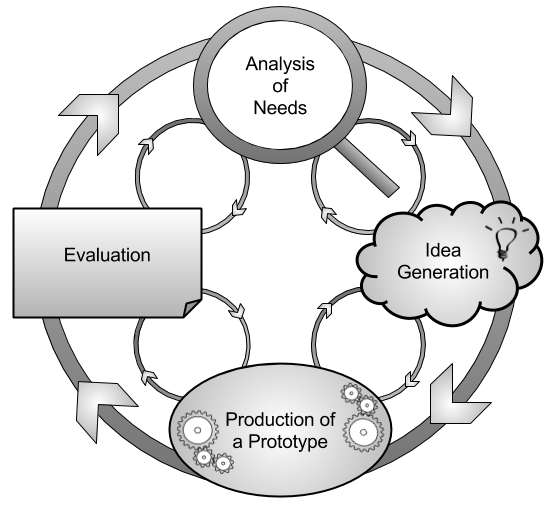
\includegraphics[width=\linewidth]{Figures/Cycle_conception.png}
                \caption{Cycle de conception}\label{fig:Cycle_conception}
            \end{minipage}
            \hfill
            \begin{minipage}{0.5\linewidth}
            \myDefautStyle
                La co-conception ou \glsdesc{ucd} est une démarche particulièrement efficace pour identifier les besoins et réguler les problèmes qui peuvent survenir sur une plateforme. Cette démarche a porté ses fruits en offrant un retour qualitatif non négligeable qui rend aujourd'hui la plateforme Poppy ErgoJr utilisable et utilisée. Cependant cette démarche est dure à étudier d'un point de vue statistique. 
            \end{minipage}
            \end{figure}\par%
            La création des activités a impliqué deux modes de conception participative. D'une part des activités conçues par l'équipe Poppy Éducation avec la contribution des enseignants et d'autre part des activités conçues par les enseignants avec un apport de l'équipe Poppy Éducation. 
            Dans le premier cas, les activités créées par l'équipe Poppy Éducation ont été modifiées à l'aide de retours d'enseignants et d'observations de situations réelles. Les activités d'initiation du livret pédagogique \gui{Apprendre à programmer Poppy ErgoJr en \sht{snap}}, qui sont détaillées plus loin~\citeS{sec:activite}, sont principalement concernées par ce mode de conception. Dans le second cas, les enseignants se sont inspirés d'activités fournies par l'équipe Poppy Éducation pour en créer de nouvelles ou ont sollicité de l'aide technique pour la mise en œuvre de leurs idées. Par ailleurs, ces activités se sont enrichies grâce à différents échanges, lors de réunions ou sur le forum. Quelques projets sont présentés plus loin.
\section{Mise en place}
    \myPhantom{paragraph}{Introduction}
        En amont de la co-création d'activités et de projets pédagogiques, nous avons analysé le programme \sht{ISN} et \sht{ICN} pour en dégager les compétences à transmettre et les modalités d'enseignement possibles~\citeS{sec:programme-officiel}. Parmi les objectifs pédagogiques visés, nous avons déterminé ceux pour lesquelles le robot ErgoJr pouvait être utile. Les activités pédagogiques qui ont été construites, seront discutées~\citeS{sec:activite} et reliées avec les objectifs du programme.\par%
        Autour du projet Poppy Éducation, de nombreuses discussions ont eu lieu avec les différents acteurs, particulièrement avec les institutions éducatives officielles, sur les fonctionnalités nécessaires au robot pour s'intégrer en salle de classe et répondre aux différents besoins.
        Suite à ces discussions et pour avoir une base sur laquelle travailler, l'équipe Poppy Éducation a développé une première version d'un kit robotique.
        Ainsi, l'évaluation et l'amélioration continues de ce kit robotique ont été menées en étroite collaboration avec les enseignants partenaires du groupe de travail et en interaction avec d'autres partenaires. Nous allons décrire ci-dessous la manière dont nous avons travaillé avec différents acteurs.
    \subsection{Les lycées}
        Le groupe de travail est composé principalement de l'équipe Poppy Éducation et d'enseignants partenaires du projet avec des interventions ponctuelles d’autres acteurs.
        Afin de créer un groupe de travail, le Rectorat de l’Académie de Bordeaux nous a mis en relation avec des enseignants de la région Aquitaine (maintenant Nouvelle-Aquitaine), proche de Bordeaux afin de faciliter les futurs déplacements. À la suite de discussions individuelles, treize enseignants de neuf établissements scolaires se sont portés volontaires pour participer au projet. Des conventions de partenariat ont été signées avec leurs établissements~\citeS{sec:adm}, et plus de 70 robots ont été prêtés à cette occasion~\citeS{sec:materiel}.
        Un panel de 9 lycées a donc participé à l'introduction de la plateforme Poppy ErgoJr.: Lycée Camille Jullian (Bordeaux), Lycée François Mauriac (Bordeaux), Lycée des Graves (Gradignan), Lycée Jean Moulin (Langon), Lycée Sud Medoc, Lycée Alfred Kastler (Talence), Lycée Saint Genès (Talence), Lycée Victor Louis (Talence), Lycée Raoul Follereau (Nevers)~\citeA{pdf:etablissements}. Ainsi, des élèves de 2\nd \sht{ICN}, et de Terminale \sht{ISN} ont pu manipuler ces robots depuis décembre 2015, dans leur classe et avec l'aide de leur enseignant. Il y a eu des projets extrêmement divers (\cf activités) basés (ou non) sur des activités existantes. Le but était d'avoir un environnement le plus proche écologiquement de leur situation d'apprentissage classique pour évaluer la plateforme en terme d'utilisabilité~\citeS{Exp:L_UX}.
        \paragraph{En présence}\label{sec:reunion}
            \subparagraph{Les réunions}
                Pour préparer les expérimentations des robots en classe par les enseignants durant l'année scolaire, une première réunion de présentation a été organisée avec les membres du groupe de travail (enseignants et membres de l’équipe Poppy Éducation) où les ingénieurs de l'équipe ont présenté des outils matériels et logiciels qu'ils avaient prototypés. Ont suivi deux demi-journées de formation à ces outils. 
                La quatrième rencontre a été consacrée à l'échange d'idées d'activités pédagogiques réalisables avec le kit pédagogique, lors de laquelle une dizaine d'idées de projets ont été présentées par l'équipe au groupe pour faire émerger des idées et suggérer des pistes de réflexions. 
                Des activités clé en main, avec conseils d’usage et solutions, d’initiation au robot Poppy ErgoJr et au langage de programmation \sht{snap} ont également été proposées aux enseignants, dans le but de continuer à les former mais aussi pour qu’ils disposent d’activités à réaliser en classe avec leurs élèves s'ils le souhaitent.
                Finalement, des robots ont été prêtés en fonction de la demande des enseignants. Il y a eu en moyenne un robot pour trois élèves et environ, quatre-vingt robots ont été prêtés la première année aux établissements partenaires.
                Une fois formés et équipés de robots, les enseignants, parfois accompagnés de membres de l’équipe selon la demande, ont mené de premières expérimentations et évaluations empiriques. Pour cela, les enseignants partenaires ont utilisé le kit robotique en classe avec leurs élèves en l'intégrant à leurs cours, à la fréquence de leur choix et en mettant en place les activités et les projets qu'ils souhaitaient~\citeS{sec:proto}. Néanmoins, il leur a été demandé de fournir des retours d'expérience et de partager les activités et les ressources éventuellement créées, ainsi que de remplir et faire remplir aux élèves des questionnaires avant et à la fin des activités robotiques.
            \subparagraph{Les visites dans les établissements}
                L'ingénieur pédagogique de l'équipe s'est déplacé régulièrement dans chaque établissement partenaire pour observer les utilisations des robots en classe et pour rédiger des comptes-rendus détaillés.
                Des déplacements occasionnels par les ingénieurs de l'équipe ont permis de tester des développements réalisés par exemple pour la connexion au réseau de l'école et l'interface de programmation applicative (\sht{api}) du robot.
        \paragraph{À distance}\label{sec:mail}
            En plus d’échanges réguliers en présentiel avec les enseignants, de nombreux échanges se sont déroulés par mail et par le forum du projet.
            \subparagraph{Les mails, visio et téléphone} Ce type de communication a réellement permis d'établir une relation de confiance et de partage sur le long terme. De nombreuses ressources ont été collectées par ce biais et, de la même façon, plusieurs difficultés ou, au contraire, ingéniosités ont pu être relayées grâce à ce vecteur. En effet, la conversation téléphonique est un outil idéal pour retranscrire des contextes, des événements ponctuels et estimer le besoin d'accompagnement sur tel ou tel sujet. D'un autre côté, les mails semblent plus adaptés pour la transmission des ressources car, à cette étape, elles sont souvent considérées par les enseignants comme \cro{un brouillon}. Cette méthode permet d'avoir une diffusion plus directe sans trop de \cro{spectateur} avant leur mise en forme et leur diffusion effective.
            \subparagraph{Le forum en ligne} Mais d'autres utilisateurs sont totalement à l'aise avec les outils publics et en ligne. Notamment, car ils ont l'avantage de faire appel directement à l'ensemble de la communauté (présente sur le forum) pour résoudre un problème, débattre d'une idée ou proposer des contenus finalisés ou en construction. Ce type de communication permet la confrontation de nombreuses personnes et participe à l'émulation autour du projet global.\par%
        \myPhantom{paragraph}{proto-activités}\label{sec:ucd_prop}
            C'est notamment par ce vecteur, le forum en ligne, qu'a été diffusé une base de 10 propositions d'activités aux enseignants. Ils étaient totalement libres de les utiliser en l'état, ou de les modifier. Ils pouvaient également laisser ce choix aux élèves. Chacun des enseignants a adapté les projets en fonction de leurs compétences initiales, donnant une grande variété de projets. Parmi les projets réalisés, 7 permettent d'illustrer une grande partie des usages rencontrés dans ces lycées, ceux-ci seront détaillés plus loin~\citeS{sec:proto-act}.
    \subsection{La seconde année}
        Durant la deuxième année, le suivi des établissements partenaires a été réduit, les enseignants étant désormais autonomes. Cependant des membres de l’équipe se sont déplacés en classe lors de rares sollicitations de leur part. Les échanges se faisaient principalement par mail ou sur le forum, certains enseignants sont venus au laboratoire de recherche pour résoudre certains problèmes techniques et quatre réunions ont été mises en place pour échanger sur les retours d’expériences. Un deuxième colloque \cro{Robotique et Éducation} a également été organisé en fin d'année.
        Les enseignants ont continué à utiliser les robots en classe et à créer de nouvelles activités pédagogiques.
        Quatre nouveaux établissements partenaires de filières d’enseignements différentes (comprenant dix nouveaux enseignants au total) ont été intégrés au projet Poppy Éducation, pour apporter de la diversité, avec de nouveaux profils d’enseignants et d’élèves. 
        L’accent a été mis sur la formation et le suivi des nouveaux enseignants ainsi que sur la création de nouvelles ressources. La diffusion a été amplifiée pour permettre au plus grand nombre de découvrir et de s’approprier les activités créées. Le site internet Poppy Éducation a été créé pour regrouper toutes les ressources et permettre aux personnes d’être autonomes sur l'utilisation des robots.
        D'autres robots ont été prêtés à d'autres établissements et acteurs, portant le nombre de kits robotiques mis à disposition à plus de 300. A noter que d’autres établissements utilisent également Poppy Éducation en achetant directement les robots au distributeur Génération Robots, mais sans suivi spécifique de la part de l’équipe.
    \subsection{Avec d'autres}\label{sec:stand}
        \paragraph{Les salons, conférences, ateliers et évènements}
            En parallèle, comme préconisé pour la construction d'une communauté open-source~\citeS{sec:com-open} nous avons assisté à de nombreux évènements de promotion des usages.
            %Comme l’explique l'étude de cas de~\citeB{ubeda2016logiciels} sur la communauté Poppy-project, 
            L'équipe Poppy-project a fait un gros travail pour diffuser et promouvoir l’exploitation du projet auprès d’un public aussi large que possible. En nous présentant comme la branche \cro{Éducation} de Poppy-project, nous avons bénéficié de son réseau. Par conséquent, nous avons régulièrement été sollicités pour participer à des événements de natures variées. La première année, dans la lignée de l'esprit Poppy-project, nous avons essayé d'accepter toutes les invitations, puis, la deuxième année, nous avons ciblé davantage nos interventions et, lorsque c’était possible, nous avons délégué à d'autres personnes de la communauté.
            Finalement, nous avons répondu favorablement à plusieurs demandes de collaboration à la suite de ces sollicitations %effectuées par des centres de formation et des structures de médiation numérique.
            Pour cela, de nombreux robots ont été prêtés en plus de ceux présents dans les lycées, des formations de formateurs, s’engageant à leur tour à former d’autres utilisateurs, ont été organisées et des événements ont été co-construits ou accompagnés par l’équipe du projet.
            Ainsi, un certain nombre d'animations, dans des forums et autres colloques, ont été réalisées. Par exemple, nous avons participé aux 'robots makers day', aux 'boussoles du numérique', à ' Connect'thouars', au 'Bordeaux Geek Festival' et à plusieurs formations à l'ESPE d'Aquitaine. %J'ai également pu participer à d'autres projets mettant en jeux les robots Poppy, comme des cours de danse, des animations dans des médiathèques, une conférence à Paris, \etc. 
            Durant toutes ces occasions, nous avons pu mettre en évidence un certain nombre de \textit{bug} qui rendait difficile la mise en place de la plateforme Poppy ErgoJr en l'état. Lors de ces événements, la présentation du kit robotique et de ses usages lors d'événements a permis d'ouvrir les discussions en rencontrant un public plus large (souvent le grand public et un public d'enseignants et de formateurs), plusieurs activités ont été prototypées. Certaines ont été reprises dans le 'livret d'activité Poppy ErgoJr, d'autres ont été mises en vidéo (\cf youtube poppy-project~\citeURL{poppy-Youtube}), ou exposées sur le forum poppy~\citeURL{poppy-forum}. Globalement, cette mise en situation et ces observations nous ont permis de dégager plusieurs hypothèses à évaluer et d'imaginer des idées d'activités à créer, spécifiques à Poppy ErgoJr.
\section{Développement}\label{sec:devellopement}
    \myPhantom{paragraph}{Introduction}
        L'analyse des programmes~\citeS{sec:programme-officiel} et des besoins
        %,cité en section précédente~\citeS{sec:ucd}, 
        a permis de déterminer plusieurs préconisations pour le développement de ce robot.
        Premièrement, pour diminuer les contraintes budgétaires, le robot devrait être peu coûteux et accessible facilement. Il serait idéal que les enseignants puissent se faire prêter les robots par des institutions. 
        Pour pallier aux difficultés d'administration des ordinateurs, l'outil devrait être utilisable sans installation de logiciels sur les ordinateurs.
        L'outil devra également faciliter la mise en pratique de la pédagogie par projet, et le travail de groupe~\citeS{sec:user_cible}. Pour s'adapter aux préférences de chaque enseignant, il faudrait que le robot soit facilement modifiable pour permettre à chacun d'entre eux de pouvoir utiliser les technologies qu'il connaît (arduino, raspberry \etc), même chose pour les langages de programmation (Python, \sht{snap}, Java \etc). Pour les ressources pédagogiques, elles devront être clé en main mais également modifiables facilement.
        Un des principal défi sera de proposer un kit robotique simple, permettant à un débutant de l'utiliser facilement pour s'initier, mais permettant aussi à une personne plus expérimentée de créer des projets complexes.
    \paragraph{En pratique}
        Après les premiers retours d'expériences formulés lors des réunions avec les professeurs partenaires de Poppy Éducation, plusieurs problèmes nous ont semblé récurrents: les activités pédagogiques étaient difficilement trouvables, il n'y avait pas assez de vidéos explicatives, l'accès aux ressources externes, telle que la documentation, était compliqué, et la langue anglaise était un obstacle à la compréhension.
        Cette tendance a été confirmée par la mise en œuvre d'entretiens semi-directifs avec des enseignants partenaires du projet depuis un an dont les objectifs étaient variés (enseignants en écoles d'ingénieurs, en lycées, en collèges) et dont les affinités avec la programmation étaient différentes. Ces entretiens avaient notamment pour objectif de mesurer la connaissance des enseignants acteurs de l'écosystème Poppy Éducation, mais aussi de mesurer leur ressenti concernant les outils mis à leur disposition.
        Les réponses les plus données lors des entretiens étaient:
        \begin{itemize}\myItemStyle
            \item Les ressources sont difficiles à trouver, voire manquantes ou indisponibles en langue française.
            \item La hiérarchie des informations présentes sur le forum est difficile à comprendre.
            \item Le contenu du forum est trop technique ou s'adresse à des utilisateurs avancés.
            \item Les ressources les plus attendues sont les activités à faire en classe, ou des idées qui leur permettent de les réaliser eux-mêmes.
        \end{itemize}\par%
        Nous avons donc décidé de créer un nouvel outil adapté aux besoins spécifiques de la communauté Poppy Éducation en nous appuyant sur ces retours d'utilisateurs, et cet outil a pris la forme d'un site internet entièrement dédié à la robotique pédagogique et en langue française. Le site poppy-Éducation.org avait vocation à devenir la nouvelle vitrine de la communauté.
        Pour ce faire, Nous avons fait circuler un document de chainstorming~\footnote{un brainstorming électronique}
        contenant plusieurs questions sur ce que devait comporter le nouvel outil Poppy Éducation.
        Voici les principaux points qui en sont ressortis, \gui{le site doit contenir \dots}: 
        \begin{itemize}\myItemStyle
          \item Les fichiers STL avec une précision des mises à jour
          \item Les modes d’emploi des robots
          \item Des articles sur la robotique
          \item La présentation de Poppy
          \item Les mises à jour des logiciels
          \item Une rubrique AIDE
          \item Une zone dédiée aux exploitations pédagogiques
          \item Une zone dédiée aux lieux pour se procurer le matériel
          \item Une zone dédiée à l'initiation programmation avec des exemples simples accessibles pour tous
          \item Une zone dédiée à la publication en Wiki pour inciter le grand public à publier les réalisations faites avec Poppy
        \end{itemize}\par%
        Une fois l'étape de recensement des items réalisée, il était nécessaire de les réagencer en rubriques, en fonctionnalités pour constituer le site.
        Pour établir ces spécifications, nous avons organisé un atelier durant lequel nous avons impliqué les utilisateurs. À l'aide de cartes en papier, chacun était invité à donner sa vision personnelle de l'architecture du site. Notre rôle était de canaliser ce processus créatif pour qu'émerge une architecture commune, répondant exactement aux besoins de la communauté. Si certaines rubriques et fonctionnalités ont changé depuis cet atelier, les principales spécifications sont restées les mêmes, et le site doit:
        \begin{itemize}\myItemStyle
          \item Être en langue française.
          \item Être agréable visuellement et user-friendly.
          \item Contenir des rubriques spécifiques à la présentation des robots et aux ressources pédagogiques.
          \item Mettre à disposition un espace dédié à la communauté.
          \item Proposer un espace d'aide comprenant les FAQ.
        \end{itemize}\par%
        Le défi était ensuite de permettre à l'ensemble de la communauté de se rassembler effectivement autour de ces outils qu'une partie créée et spécifiée elle-même.